\chapter{Conception de la plateforme}

\section{Introduction}

L'objectif de ce travail, en premier lieu, est d'avoir un ensemble de données
composé d'images d'environnement avec un certain nombre de distances qui
représentent  les écarts respectifs entre la position de l'appareil permettant
de prendre chaque image et les obstacles qui sont y visibles.

Afin d'atteindre ce but nous avons vu la nécessité de fabriquer une machine mobile
permettant l'acquisition de ces données d'une manière automatique. La machine que
nous avons réalisé nous facilite la tâche et accélère énormément le rythme du travail.
De ce fait, nous pouvons obtenir une quantité importante de données dans un temps
réduit.

Cette machine possède une capacité limitée de navigation automatique, mais
elle peut être télécommandée par un ordinateur à travers une connexion sans fil
entre le programme qui s'exécute sur l'ordinateur et les programmes qui ordonnent
la machine. L'ensemble de ces programmes avec le matériel forment un système
qui a pour rôle de collecter les données nécessaires pour l'étape de
l'apprentissage automatique.

Le système est composé d'une partie matérielle et d'une autre logicielle. Chaque
partie sera présentée à part en montrant les détails de son fonctionnement.

\section{La partie matérielle}

La construction physique du robot est composée d'une carcasse et de plusieurs
parties électroniques, chaque partie offrant au moins une fonctionnalité
élémentaire. Les parties principales sont :

\begin{itemize}
  \item quatre moteurs de courant continu,
  \item un pilote de moteurs \keyword{L298N},
  \item des capteurs ultrasoniques \keyword{HC-S04},
  \item un moteur servo \keyword{TowerPro SG90},
  \item un capteur de température (et d'humidité) \keyword{DHT22},
  \item un microcontrôleur \keyword{Arduino Mega 2560},
  \item un appareil équipé du système d'exploitation \keyword{Android},
  disposant d'une camera RGB et d'un port USB qui permet la connexion en série
  (dans notre cas, nous avons utilisé un téléphone \keyword{Samsung Galaxy Note 2})
  \item une source d'alimentation électrique qui peut fournir une intensité de
  courant suffisante pour faire fonctionner les moteurs et les capteurs (nous
  avons utilisé une banque d'alimentation électrique combinée avec des piles).
\end{itemize}

\subsection{Le pilotage des moteurs}

Un moteur de courant continu tourne dans une seule direction à la fois. Cette
direction est déterminée par le sens du courant traversant la bobine interne
du moteur. La direction de la rotation peut être inversée seulement en inversant
le sens du courant électrique. De plus, l'intensité de ce courant détermine la
vitesse à laquelle ce moteur tourne.

\begin{figure}[h]
\begin{center}
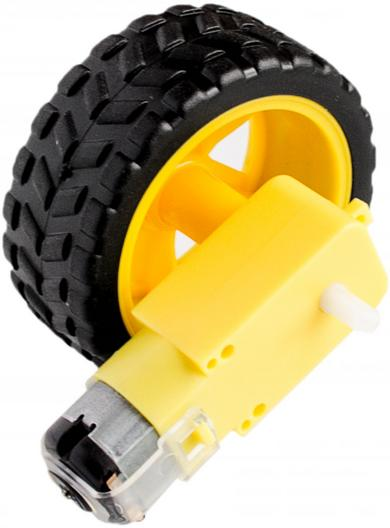
\includegraphics[width=0.2\textwidth]{DC_motor_wheel}
\caption{Le moteur de courant continu utilisé avec la roue}
\end{center}
\end{figure}

Pour pouvoir manipuler ces paramètres (le sens et la vitesse de la rotation), il
faut utiliser un pilote de moteurs comme \keyword{L298N}. Ce module peut contrôler
deux moteurs indépendamment, chacun dans un sens et à une vitesse donnée. Cependant, il est
aussi capable de gérer plus de deux moteurs, à condition qu'ils soient distribués
en deux groupes de telle manière que tous les moteurs du même groupe fonctionnent
par les mêmes paramètres.

Dans ce travail, nous avons eu recours à quatres moteurs
(pour supporter le poids du véhicule), chaque paire étant considérée comme un
seul groupe et située dans un côté du véhicule (droite ou gauche).
Les moteurs d'un côté tournent toujours dans le même sens avec la même vitesse.
La variance du sens entre les deux côtés détermine le type de mouvement : si
tous les moteurs tournent dans le même sens, alors le robot avance ou recule
selon le sens de la rotation, et si les moteurs des différents côtés tournent dans
des sens différents, alors le robot tourne autour de lui-même.

\begin{figure}[h]
\begin{center}
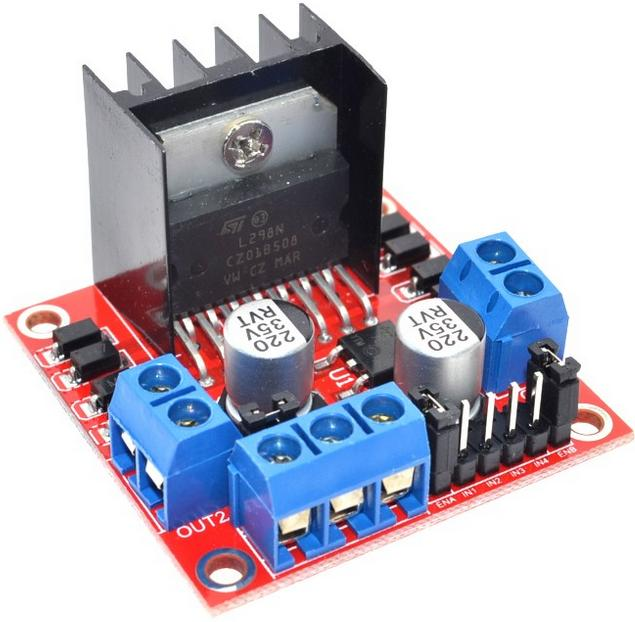
\includegraphics[width=0.3\textwidth]{L298N}
\caption{Le contrôleur de moteurs L298N}
\end{center}
\end{figure}

\subsection{La mesure de distances}

Les capteurs ultrasoniques sont des composants qui permettent l'envoi et la
réception du signal ultrasonique. En effet, ils sont utilisés pour le calcul
de la distance d'un objet. Pour ce faire, le capteur est commandé afin d'émettre
un signal dans une direction spécifiée. Si le signal ne frappe aucun objet avant de
s'affaiblir, il sera perdu et la distance ne pourra pas être calculée; sinon il
retournera au capteur à qui il notifiera le circuit commandant par la réception.
Par la suite, le circuit peut calculer la différence entre les instants d'émission
et de réception et utilise cette durée pour estimer la distance en connaissant
la vitesse du son dans l'air. La distance $d$ ($m/s$) est estimée par la formule suivante :

\begin{equation}
  d = t \times c \div 2,
\end{equation}

où $t$ est le temps écoulé en secondes entre l'envoi et la réception du signal,
et $c$ est la vitesse du son dans l'air sec et est approximée par la formule :

\begin{equation}
  c = 0.6 \times T + 331.4,
\end{equation}

avec $T$ la température de l'environnement en Celsius ($ ^\circ C$).

Afin de déterminer la température de l'air, nous avons utilisé le capteur
\keyword{DHT22} qui permet un relèvement de la température chaque $2$
secondes avec une haute précision (la marge d'erreur est seulement $\pm 0.5 ^\circ C$).

Ce capteur fonctionne en mode numérique. Il est activé seulement quand il reçoit
un signal approprié. Il renvoie le résultat à travers le même port au circuit
instantanément après avoir pris les mesures nécessaires.

\begin{figure}[h]
\begin{center}
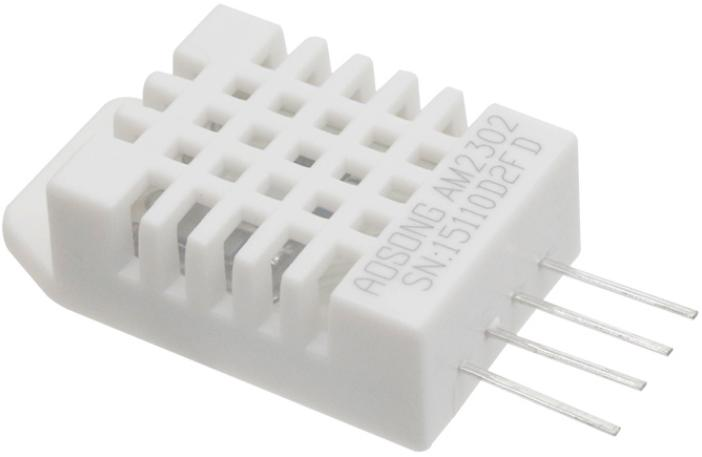
\includegraphics[width=0.25\textwidth]{DHT22}
\caption{Le capteur de la température DHT22}
\end{center}
\end{figure}

En outre, les capteurs d'ultrason opèrent sur une seule direction à la fois. Si
nous voulons avoir un ensemble de distances pour les différents obstacles éventuels
visibles dans le champ de vision du robot, nous avons besoin de plusieurs capteurs.

Mieux encore, on peut n'en utiliser qu'un seul et le faire tourner sous plusieurs
angles afin de couvrir la zone de vision.
Pour cela, il faut monter le capteur ultrasonique sur le bras d'un \keyword{servomoteur}.
Ces moteurs ont la capacité de déplacer leur bras par des angles exacts compris
généralement entre $0^\circ$ et $180^\circ$. Le circuit de contrôle envoie l'angle
d'inclinaison du bras au servomoteur qui effectue cette opération mécanique rapidement.
Nous avons utilisé le servomoteur \keyword{TowerPro SG90} pour cette tâche.

\begin{figure}[h]
\begin{center}
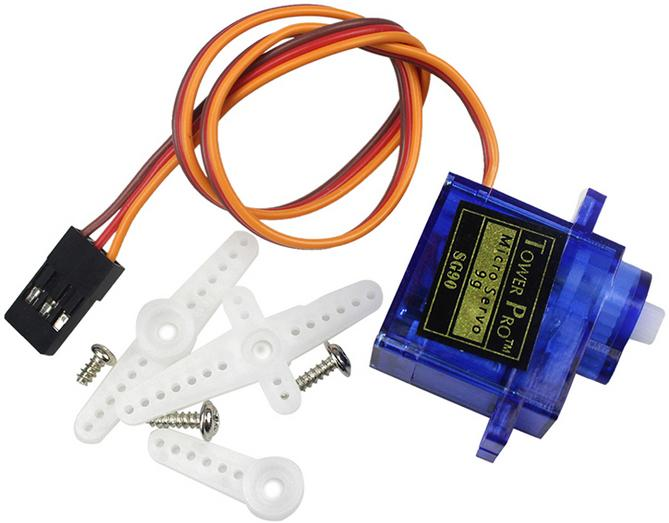
\includegraphics[width=0.3\textwidth]{SG90}
\caption{Le servomoteur TowerPro SG90}
\end{center}
\end{figure}

\subsection{Le contrôle des composants}

Afin de contrôler tous les modules précédents, il nous faut un microcontrôleur.
Dans ce travail, nous avons utilisé une version compatible avec le
microcontrôleur \keyword{Arduino Mega 2560}.

Nous avons connecté les ports de données de ce microcontrôleur aux autres
composants (le pilote de moteurs, le capteur ultrasonique, le capteur de la
température et le servomoteur) en utilisant des câbles compatibles après avoir
placé tous ces modules dans leurs positions respectives. Par la suite, il sera
chargé par un programme permettant de gérer continuellement les autres modules
par l'envoi de commandes ou par la réception d'informations.

\begin{figure}[h]
\begin{center}
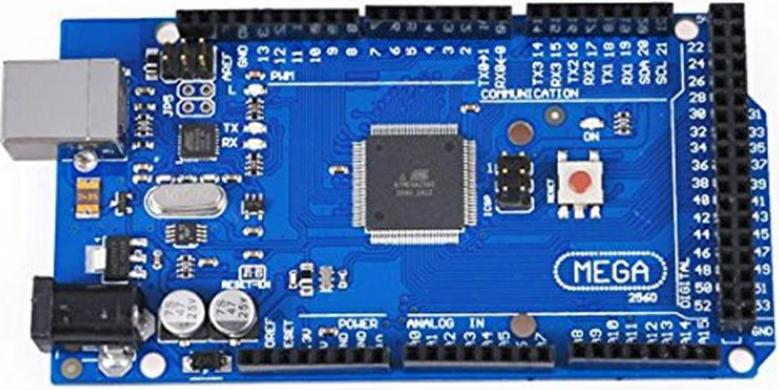
\includegraphics[width=0.4\textwidth]{ArduinoMega2560}
\caption{Une version compatible avec le microcontrôleur Arduino Mega 2560}
\end{center}
\end{figure}

Il y a deux types de ports : les \keyword{ports numériques} à lecture et
écriture, et les \keyword{ports analogiques} à lecture seule. Certains ports
numériques supportent \keyword{la modulation de largeur d'impulsion} et donc peuvent
émettre un signal composé d'une succession d'états discrets de <<tout ou rien>>
pendant une unité de temps dont la fréquence est choisie par le programme.

Étant donné que les performances du microcontrôleur sont très limitées, nous
devons le connecter à un appareil plus puissant en termes de vitesse
de calcul et de capacité en mémoire, et disposant d'autres options comme la
mise en réseau. Afin de satisfaire ces besoins, nous avons intégré le téléphone
intelligent \keyword{Samsung Galaxy Note 2} comme partie du robot en le connectant
par un cable USB avec le microcontrôleur. Cela permet d'établir une connexion en série entre
ces deux appareils, après avoir développé une application s'exécutant
sur le téléphone et permettant l'échange d'informations avec le microcontrôleur
en même temps qu'avec l'ordinateur hôte.

\begin{figure}[H]
\begin{center}
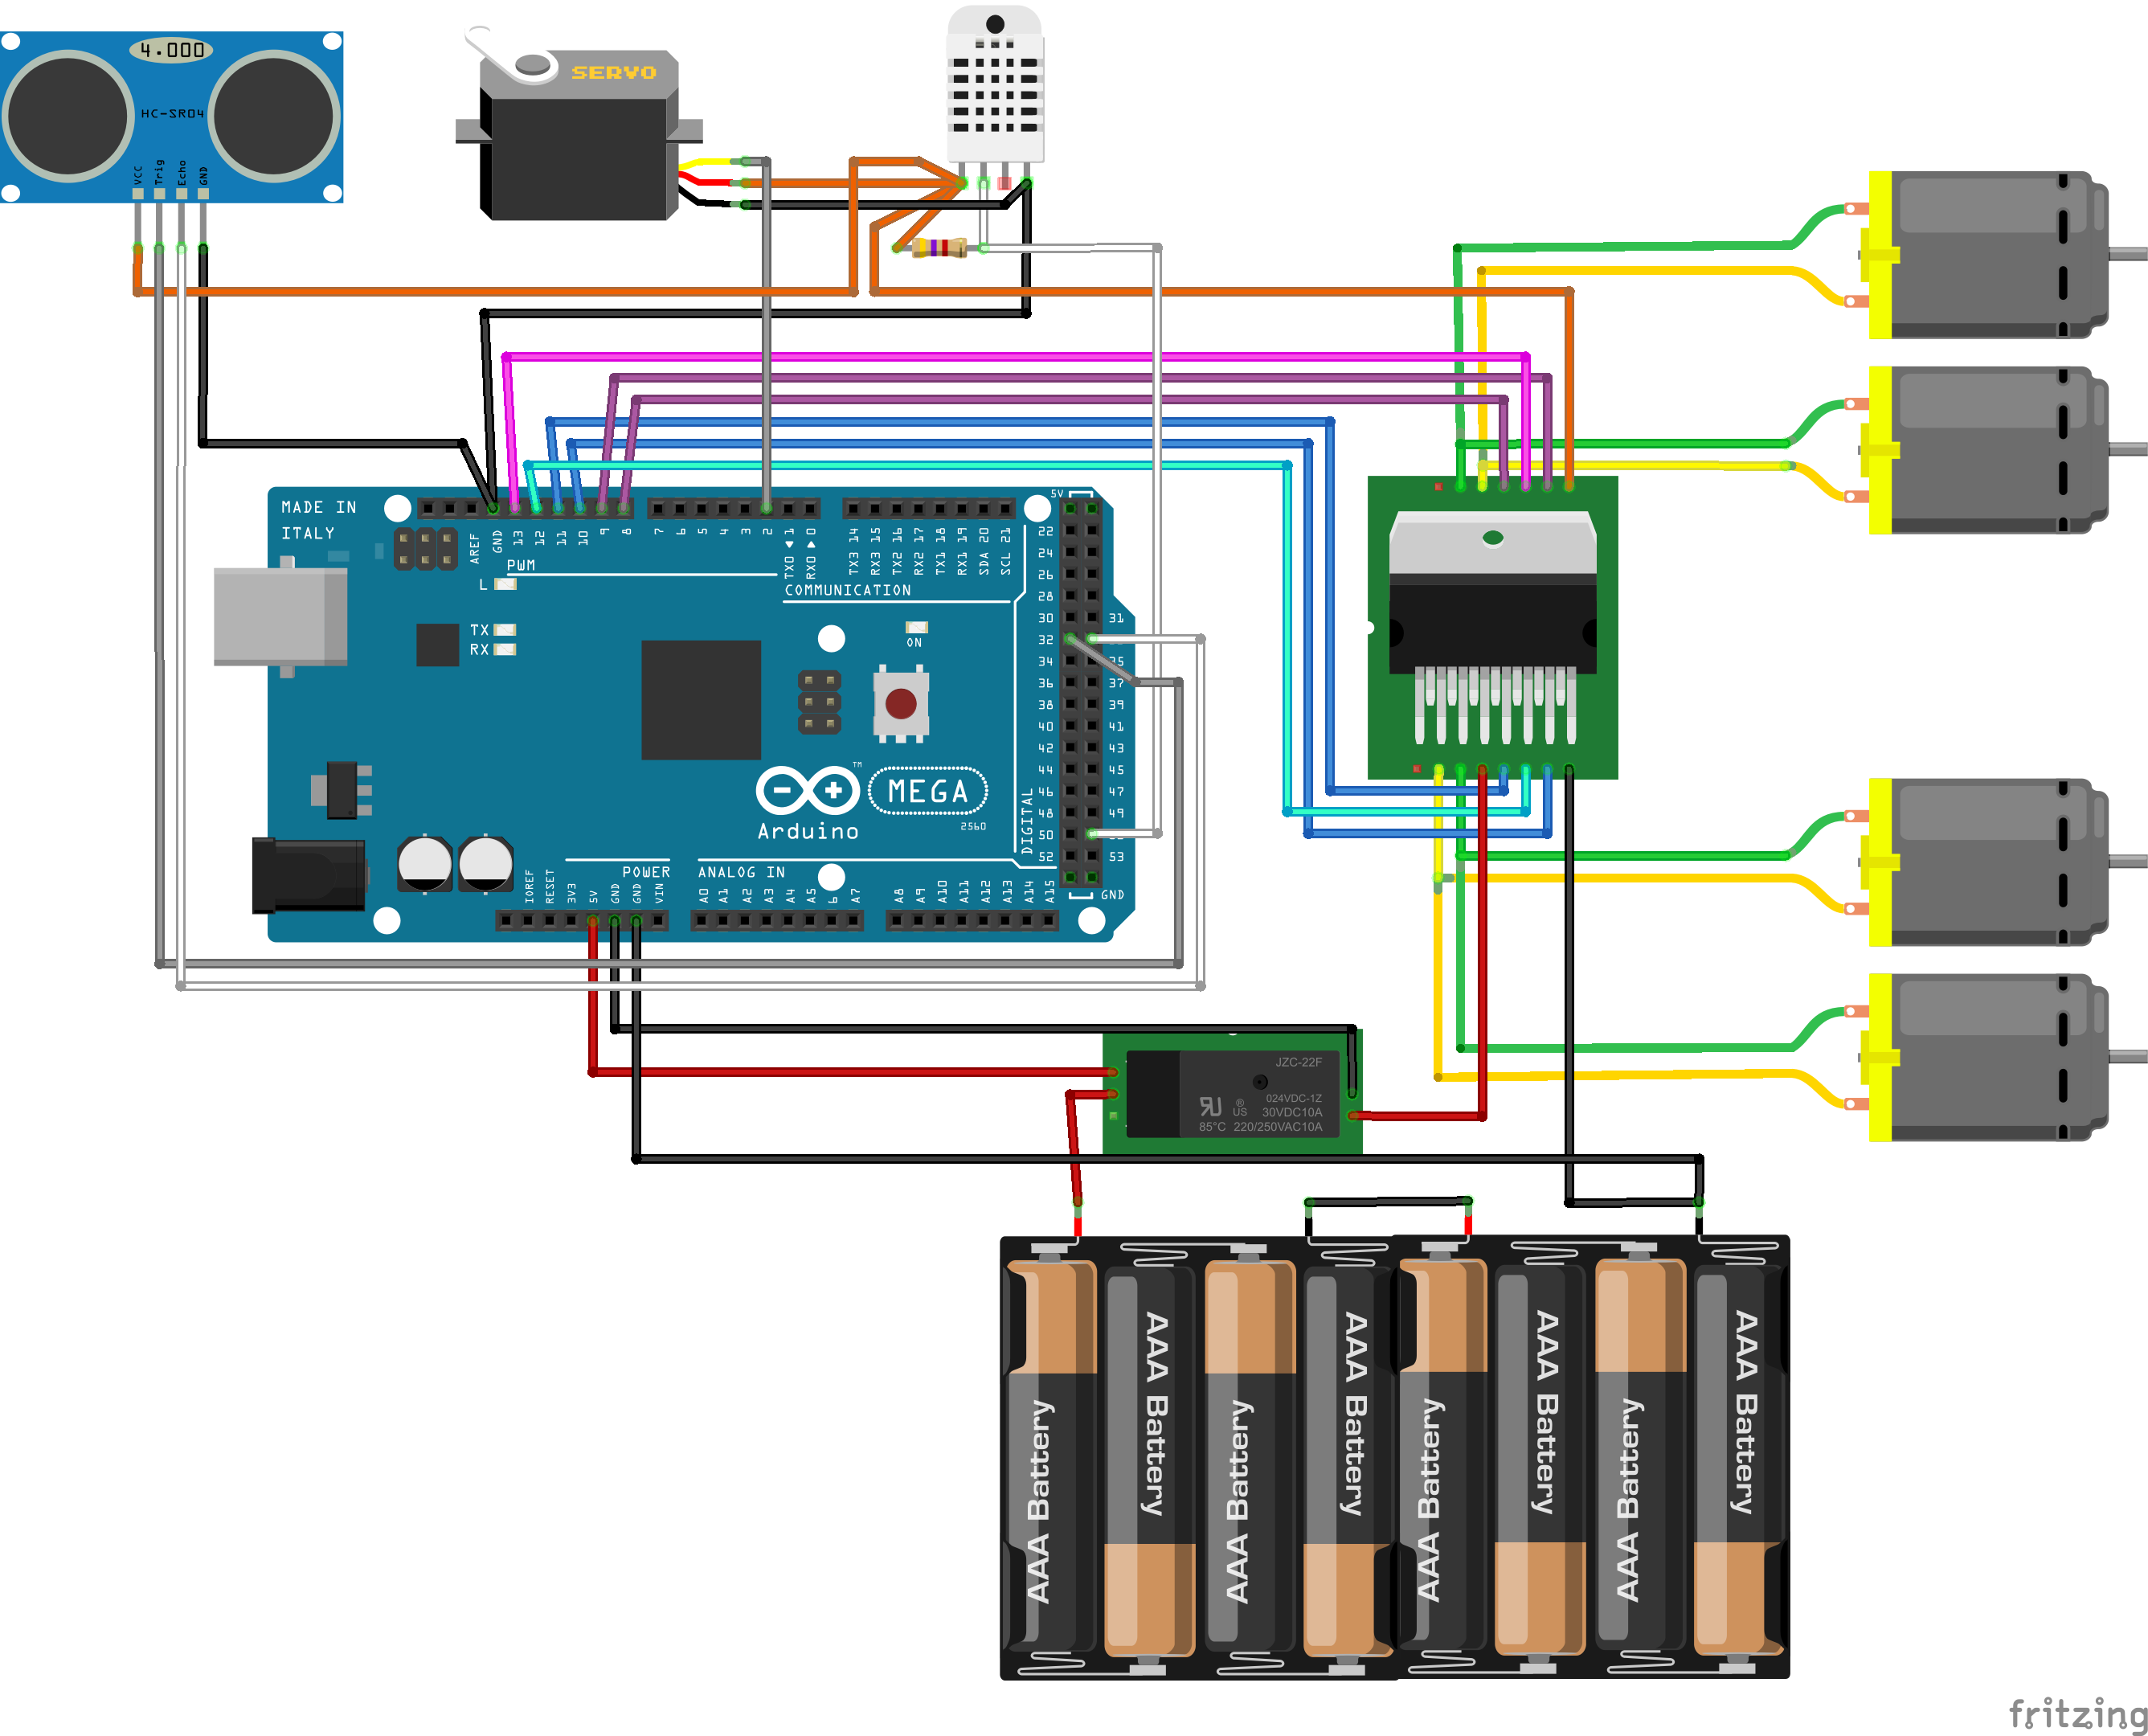
\includegraphics[width=0.8\textwidth]{DistancesRobotCircuit}
\caption{Le schéma des connexions entre les modules du robot}
\end{center}
\end{figure}

Jusque là, nous avons présenté les composants matériels nécessaires pour la
construction du robot et la manière dont ils sont utilisés en indiquant la
fonctionalité de chacun d'eux. Dans la partie suivante nous présenterons les
logiciels développés pour chaque plateforme et nous expliquerons leur fonctionnement
ainsi que leur intercommunication qui permettent la gestion du robot.

\begin{figure}[h]
\begin{center}
  \begin{subfigure}{0.49\textwidth}
    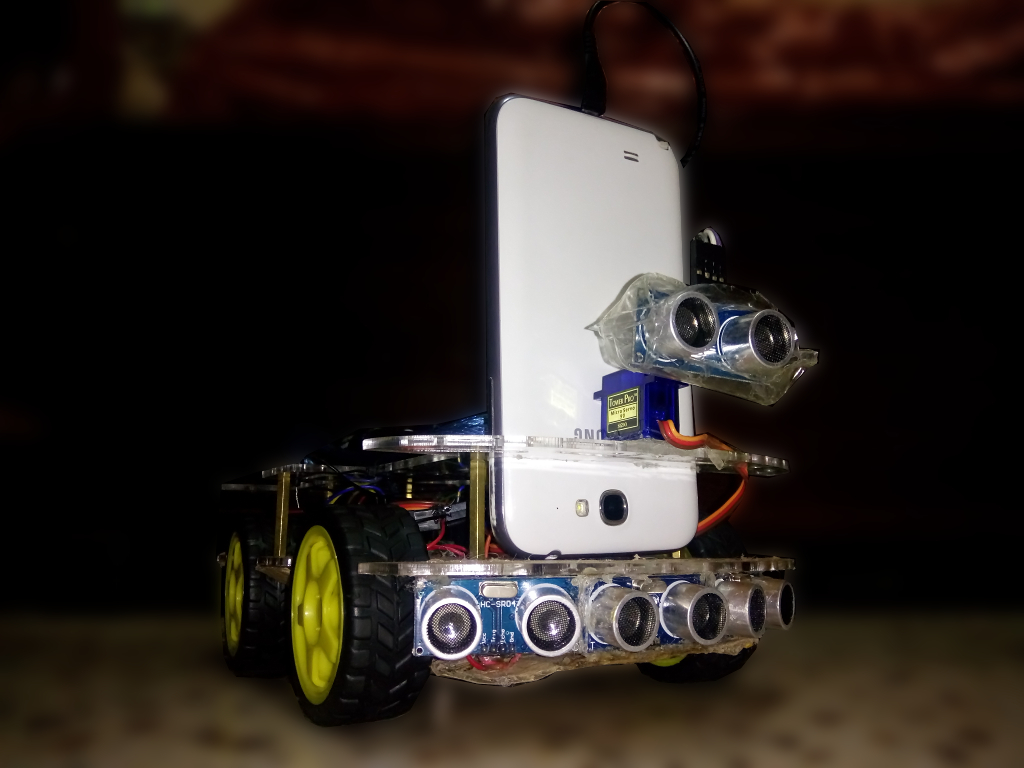
\includegraphics[width=\textwidth]{Distances_robot_front}
    \caption{Vue de face}
  \end{subfigure}
  \hfill
  \begin{subfigure}{0.49\textwidth}
    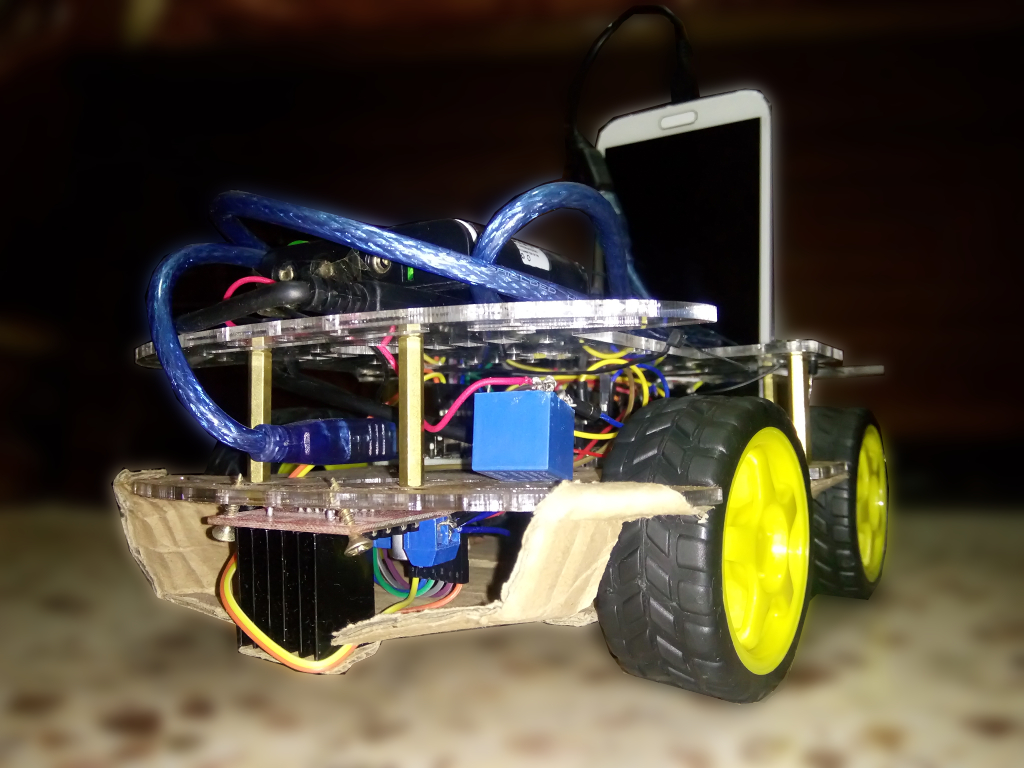
\includegraphics[width=\textwidth]{Distances_robot_back}
    \caption{Vue arrière}
  \end{subfigure}
  \caption{Des photos du robot}
\end{center}
\end{figure}

\section{La partie logicielle}

L'ensemble des composants du robot est géré directement par deux logiciels, l'un
s'exécute sur le microcontrôleur, et l'autre sur le téléphone. Ce dernier
envoie des commandes à l'autre qui contrôle directement le matériel.

\subsection{Le programme du microcontrôleur}

C'est un programme répétitif, testant à chaque fois s'il y a
une commande reçue par le téléphone à travers la connexion en série. Si c'est le cas,
il teste le nom de la commande pour savoir quelle action il faut exécuter.
Une fois que l'action et ses paramètres éventuels sont déterminés, un signal
approprié est envoyé au module correspondant qui exécute cette action et renvoie
éventuellement une réponse. Cette réponse qui est déterminée par l'environnement
est capturée par le microcontrôleur et traitée à ce niveau avant de la propager
au téléphone.

Ce programme reconnaît plusieurs commandes, chacune étant représentée par un
caractère. Si la commande nécessite un paramètre (par exemple le changement de la
puissance des moteurs), le caractère de la commande est suivi par une chaîne de
caractères contenant la valeur du paramètre. Cette valeur est toujours un nombre
entier.

Si l'action performée en reconnaissant une commande retourne un résultat (par
exemple la température), il est envoyé au téléphone comme une chaîne de
caractères. Le téléphone traîte le résultat comme nous détaillerons dans la prochaine partie.

L'algorithme suivant présente le fonctionnement général du programme du
microcontrôleur. Il est constitué d'une boucle infinie (c'est-à-dire qu'elle
s'exécute tant que l'appareil est allumé) qui attend la réception d'une commande
et puis teste son type afin d'effectuer l'action nécessaire.

\smallskip

\begin{algorithm}[h]
\caption{Le programme du microcontrôleur}
\BlankLine
\While{le microcontrôleur est allumé}{
  \If{il y a une commande reçue}{
    \Switch{la commande}{
      \Case{distances}{
        Mesurer les distances et les envoyer\;
      }
      \Case{mouvement}{
        Tourner/Arrêter les moteurs\;
      }
      \Case{température}{
        Prendre la température et l'envoyer\;
      }
      \Case{puissance}{
        Ajuster la puissance des moteur\;
      }
    }
  }
}
\end{algorithm}

La commande de distance ordonne au microcontrôleur d'envoyer des signaux
successifs au servomoteur pour le faire tourner d'un angle à chaque fois ($10$ degrés
dans notre cas). La durée entre l'envoi d'un signal et le suivant est fixée dans
le programme afin de réserver la durée nécessaire pour l'opération mécanique (qui
est la rotation du bras du servomoteur). En même temps, la distance vers le
premier obstacle est mesurée à chaque angle par l'envoi d'un autre signal au capteur
de distances monté sur le servomoteur. La mesure de distance n'est pas toujours
possible : si l'objet est très loin (plus de $4.5m$) ou si sa surface est inclinée
ou irrégulière, alors l'ultrason envoyé sera perdu et la distance ne peut pas être
déterminée. Dans ce cas, une valeur constante et grande sera mise à la place de la
distance réelle pour indiquer qu'elle est inconnue. L'ensemble de distances est
transféré par la suite au téléphone par le biais de la connexion en série.

Les commandes de mouvement sont les quatre commandes de direction (avancer, réculer
tourner à droite et tourner à gauche) et la commande d'arrêt. Lors de la
réception de la commande d'arrêt, le microcontrôleur ordonne au pilote des moteurs
de couper le courant passant dans tous les moteurs, ce qui cause leur arrêt. Dans
le cas de la commande d'avancement ou de recul, tous les moteurs sont alimentés
par un courant de même sens dont un sens provoque l'avancement et l'autre cause
le recul. Le même principe s'applique pour tourner le robot, sauf que le courant
passant par les moteurs d'un côté est l'inverse de celui passant par les moteurs
de l'autre côté.

La commande de relèvement de la température est exécutée pour
mettre à jour la valeur de celle ci dans la mémoire et l'afficher à l'utilisateur.
Cette valeur est indispensable pour le calcul de la vitesse du son dans l'air
dans l'environnement courant. Le relèvement est fait par l'envoi d'un signal spécial
au capteur qui renvoie la température courante au microcontrôleur.

Toutes les actions citées précédement ne sont exécutées que à la réception de
la commande correspondante à partir de l'application du téléphone que nous expliquerons
son fonctionnement dans ce qui suit.

\subsection{L'application du téléphone}

Elle a pour rôle de commander
le microcontrôleur et d'en recevoir des informations. Les informations
sont utilisées pour faire des calculs et prendre des décisions sous
forme d'actions. Certaines sont également envoyées au logiciel qui s'exécute sur
l'ordinateur. De plus, elle prend périodiquement des images en utilisant la camera
du téléphone.

L'application envoie une commande de température après chaque intervalle de temps
($2$ secondes) au micrôcontrolleur. Dès la réception de sa valeur, elle met à
jour son interface graphique et l'envoie à l'ordinateur.

De même, l'application envoie la commande de distances et prend une photo périodiquement
(chaque $0.3$ seconde). Les distances retournées et la photo prise sont sauvegardées
temporairement dans deux files, chaque file correspondant à un type d'objets.
\`A chaque fois, un élément de chaque file est défilé et selon le mode
de la capture et la fréquence de la sauvegarde (qui est fixée à $1$ instance de
données par seconde), ces éléments peuvent être enregistrées de façon permanente
dans la mémoire externe.

L'envoi des commandes de mouvement dépend directement du mode de la navigation.
Si le mode est automatique, l'envoi est exécutée après chaque intervalle de temps
(qui est égale aussi à $0.3$ seconde). Dans ce cas, l'application décide quelle
commande il faut envoyer en utilisant les distances précédents.
Si le mode est manuel, l'envoi est effectué seulement quand l'application reçoit
un ordre explicite de l'utilisateur.

La commande de changement de puissance est toujours exécutée seulement
à l'ordre de l'utilisateur. Elle contient la valeur de la puissance qui
est un nombre entier définit sur l'intervalle $[0-255]$. Cette valeur est initialisée
par défaut à $127$.

Cette application acte également comme un pont entre l'ordinateur et le microcontrôleur
en utilisant deux types de connexions : une connexion en série par câble entre
le téléphone et le microcontrôleur, et une autre sans fil par Bluetooth entre
le téléphone et l'ordinateur. Les connexions restent toujours ouvertes
mais les transferts n'ont lieu qu'à certains moments. Ces transferts peuvent
se faire dans les deux sens et sont soit périodiques soit apériodiques selon l'action.

Les actions périodiques sont :
\begin{itemize}
  \item le relèvement de la température de l'air dans l'environnement,
  \item le choix de la direction de la navigation,
  \item la sauvegarde des données sur le périphérique du stockage externe (la carte mémoire).
\end{itemize}

\bigskip

Les actions apériodiques sont :
\begin{itemize}
  \item l'envoi de commandes de mouvement issues de l'utilisateur,
  \item le changement de la puissance des moteurs,
  \item le lancement et l'arrêt de la capture et de la navigation.
\end{itemize}

\subsection{Le logiciel de l'ordinateur}

Il offre une interface qui permet à l'utilisateur
de contrôler le robot à distance et de garder un œil sur son état. Il affiche la
température de l'air où se situe le robot et le nombre de données capturées et
sauvegardées sur la mémoire permanente. Il permet aussi de signaler quelques
erreurs causées par le matériel comme le dysfonctionnement de la camera.

\begin{figure}[h]
\begin{center}
  \begin{subfigure}{0.4\textwidth}
    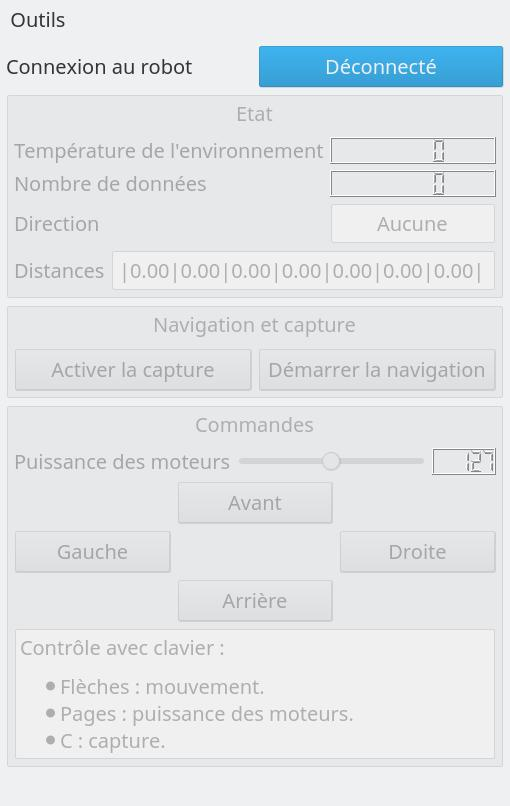
\includegraphics[width=\textwidth]{ComputerControler}
    \caption{\'Etat \textbf{déconnecté}}
  \end{subfigure}
  \hspace{2em}
  \begin{subfigure}{0.4\textwidth}
    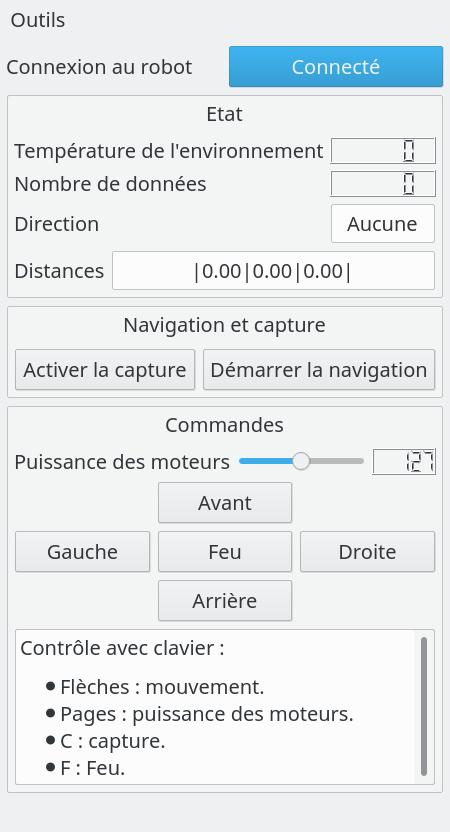
\includegraphics[width=\textwidth]{ComputerControler_connected}
    \caption{\'Etat \textbf{connecté} avec navigation}
  \end{subfigure}
  \caption{L'interface principale du logiciel d'ordinateur}
\end{center}
\end{figure}

Le logiciel permet de guider de façon directe le robot en envoyant des commandes
de direction (avant, arrière, droite et gauche) ou un signal de
navigation automatique. Il permet également de changer la puissance des moteurs
et d'activer ou de désactiver la sauvegarde de données capturées.
La sauvegarde peut être effectuée indépendamment
du mode de navigation, c'est-à-dire qu'elle peut être activée sans que la
navigation soit automatique et vice versa.

Les commandes de mouvement et de sauvegarde peuvent être activées par les
boutons existant sur l'interface ou par des touches de clavier. Les instructions
permettant de guider la machine par n'importe quelle méthode sont clairement visibles
sur l'interface.

Ce logiciel offre une autre interface qui a pour fonction de visualiser les
données collectées en affichant à la fois une photo capturée avec les distances
respectives en mètres.

\begin{figure}[H]
\begin{center}
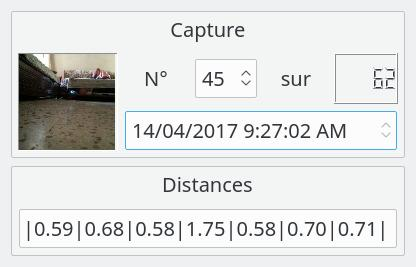
\includegraphics[width=0.4\textwidth]{CapturesViewer}
\caption{L'interface de la visualisation des données}
\end{center}
\end{figure}

\section{La collecte et le traitement des données}

Après avoir allumé le robot et lancé les programmes nécessaires, il peut commencer
à effectuer la tâche d'acquisition. Il se déplace et prend périodiquement une image
de taille $480 \times 640$, ensuite il coupe ses marges haute et basse par un
déplacement de $80$ pixels sur chaque marge, ce qui aboutit à une image carrée
de $480 \times 480$ pixels. La taille de l'image est par la suite réduite à
$96 \times 96$ pixels pour des raisons d'économisation de l'espace de stockage
et d'optimisation des calculs de l'apprentissage automatique qui sera effectué
ultérieurement. Chaque image est sauvegardée comme un fichier qui porte comme
nom un préfixe (\texttt{IMG\_}) suivi par un identificateur numérique généré
au moment de la capture (l'\keyword{époque}\footnote{Elle représente le nombre de
millisecondes passées depuis le premier janvier 1970 à minuit dans le temps
universel coordonné (UTC).}). En même temps, dans un autre fichier, les distances
correspondant à chaque image sont enregistrées avec l'identificateur de cette
dernière, chaque instance étant écrite sur une ligne. Le nombre de distances
est fixé à $3$ par image. Si la distance ne peut être mesurée, alors une valeur
constante ($9.99$) est insérée pour indiquer que la distance est manquante.

\section{Conclusion}

Dans chaque problème d'apprentissage automatique, un ensemble de données considérable
est nécessaire pour pouvoir effectuer cette tâche. Cette nécessité nous a mis devant
deux choix : utiliser un ensemble de données prêt où les données sont collectées
et traitées par d'autres personnes, ou bien construire notre propre ensemble en
utilisant nos propres outils que nous devons développer nous-mêmes.

Nous avons choisi la deuxième méthode. De ce fait, nous avons
fabriqué le robot dont nous avons décrit la construction matérielle et la
programmation au niveau logiciel. Il nous a permis de collecter les images
prises au niveau de sa vision et les distances des obstacles éventuels dans
chaque image.

Dans le chapitre suivant, nous allons exploiter ces données grâce à
un apprentissage automatique supervisé en utilisant la méthode de
réseaux de neurones convolutionels.
